\documentclass{article}

\usepackage{custom}

\title{Creating Heterogeneous Simulations by Interoperating SST with Hardware Description Frameworks}

\author{
  Sabbir Ahmed \\
  Booz Allen Hamilton \\
  ahmed\_sabbir@bah.com
}

\begin{document}
  \maketitle

  \begin{abstract}
    Implementing new computer system designs involves careful study of both programming models and
    hardware design and organization, a process that frequently introduces distinct challenges.
    Hardware and software definitions are often simulated to undertake these difficulties.
    Structural Simulation Toolkit (SST), a parallel event-based simulation framework that allows
    custom and vendor models to be interconnected to create a system simulation \cite{sst}, is one
    such toolkit. However, SST must be able to support models implemented in various hardware-level
    modeling languages (PyRTL, SystemC, Chisel, etc.) and hardware description languages (VHDL,
    Verilog and SystemVerilog). Establishing communication with these modules would allow SST to
    interface numerous existing synthesizable hardware models. SST Interoperability Toolkit (SIT) is
    a toolkit developed to provide interoperability between SST and other frameworks. SIT aims to
    achieve this capability in a modular design without interfering with the kernels by concealing
    the communication protocols in black box interfaces.
    % This project includes a demonstration of the
    % interoperability by simulating a vehicular traffic intersection with traffic lights driven by
    % SystemC and PyRTL processes.
  \end{abstract}

  \section{Introduction}  
  The increasing size and complexity of systems require engineers heavily rely on simulation
  techniques during the development phases. Typically, simulations of these complex systems require
  both custom and off-the-shelf logic functionality in application-specific integrated circuits
  (ASIC) or field programmable gate arrays (FPGA). High-level commercial tools simulate and model
  these components in their native environments. On the other side, developers create the register
  transfer level (RTL) models representing the systems to simulate them with computer-aided design
  (CAD) tools and test benches. These duplicative strategies require a method that simulates the
  entire system in one heterogeneous model.

  SST is an event-based framework that has the capabilities to simulate not only functionality but
  timing, power or any other information required. Each SST components can be assigned a clock to
  synchronize tasks. They communicate events with each other via SST links by triggering their
  corresponding event handlers. The SST models are constructed in C++ and consist of the
  functionality of the element, the definition of each links' ports and the event handlers. The
  models are connected and initialized through the SST Python module.

  % PyRTL and SystemC are platforms that deliberately mimic hardware description languages in Python
  % and C++ respectively. These system-level modeling languages provide event-driven simulation
  % kernels along with signals, events and synchronization primitives.

  Implementing a heterogeneous system to synchronize signals and events between the frameworks would
  allow the developers to work cooperatively and efficiently.

  % This paper provides a demonstration of
  % the interoperability by simulating a vehicular traffic intersection with traffic lights driven by
  % PyRTL and SystemC processes.

  Note: For the sake of simplicity and consistency in the nomenclature, the languages, toolkits or
  libraries in the following categories will be simply labeled as ``hardware description
  frameworks'', ``HDL'' or ``external HDL'':
  \begin{itemize}
    \item hardware description languages (SystemVerilog, Verilog, VHDL, etc.)
    \item system-level modeling languages (Chisel, PyRTL, SystemC, etc.)
  \end{itemize}

  \section{Black Box Interface}
  SIT conceals the communication implementation in black box driver files. This strategy allows the
  SST component to connect with the HDL processes via SST links as if they were a component itself.

  \begin{figure}[!h]
    \centering
    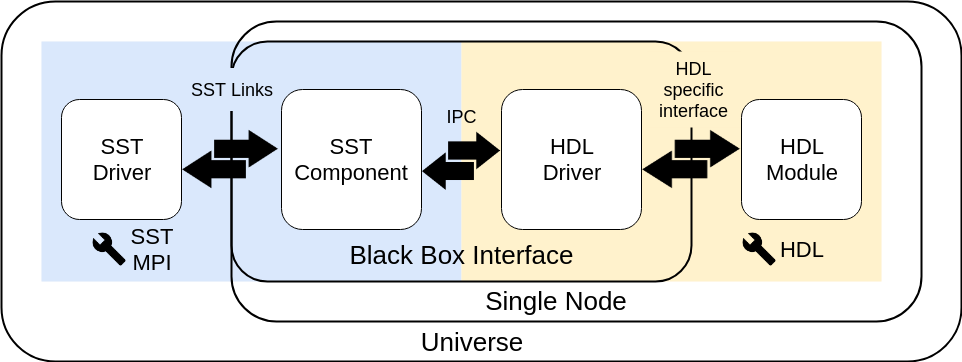
\includegraphics[width=6.5in]{diagrams/comm.png}
    \caption{Components of SIT}
    \label{fig:comm}
  \end{figure}

  The interface consists of:
  \begin{enumerate}
    \item an HDL driver
    \item an SST component
  \end{enumerate}

    \subsection{SST Component}
    The black box SST component consists of the following methods:
    \begin{itemize}
      \item Constructor
      \item \texttt{void setup()}
      \item \texttt{bool tick(SST::Cycle\_t)}
      \item \texttt{void handle\_event(SST::Event *)}
    \end{itemize}

      \subsubsection{Constructor}
      The constructor assigns the component links and declares the member attributes and sizes.

      \subsubsection{setup}
      The overridden method forks and synchronizes with its corresponding HDL driver child process.

      \subsubsection{tick}
      The overridden method simply returns \texttt{false} to prevent any clock delays.

      \subsubsection{handle\_event}
      The method is a custom event handler that receives SST String Events and parses the string
      buffer for transfer. The first 2 characters of the string are flags for the HDL driver to
      continue sending and receiving data respectively. The rest of the data is prepended with the
      HDL driver power state flag and sent to the child process via the selected communication
      protocol.

    \subsection{HDL Driver}
    Each HDL modules must have their corresponding driver file to interoperate with the SST kernel
    within the black box interface. The language or framework must be able to bind to interprocess
    communication (IPC) ports to send and receive data. The driver must be compiled separately from
    the SST component.

    \subsection{Boilerplate Code Generator}
    The toolkit includes a Python class that generates the boilerplate code required for the black
    box interface.

    The generator expects the following inputs:
    \begin{itemize}

      \item ipc - method of interprocess communication protocol

      \item module - SST element component and HDL module name

      \item lib - SST element library name

      \item width\_macros (default: None) - mapping of signal width macros to their integer values. An HDL module may declare constants or user-inputted variables in their implementation to determine signal widths.

      \item module\_dir (default: "") - directory of HDL module

      \item lib\_dir (default: "") - directory of SIT library

      \item desc (default: "") - description of the SST model

      \item driver\_template\_path (default: "") - path to the black box-driver boilerplate

      \item component\_template\_path (default: "") - path to the black box-model boilerplate

    \end{itemize}

  \section{Communication}

  \begin{figure}[!h]
    \centering
    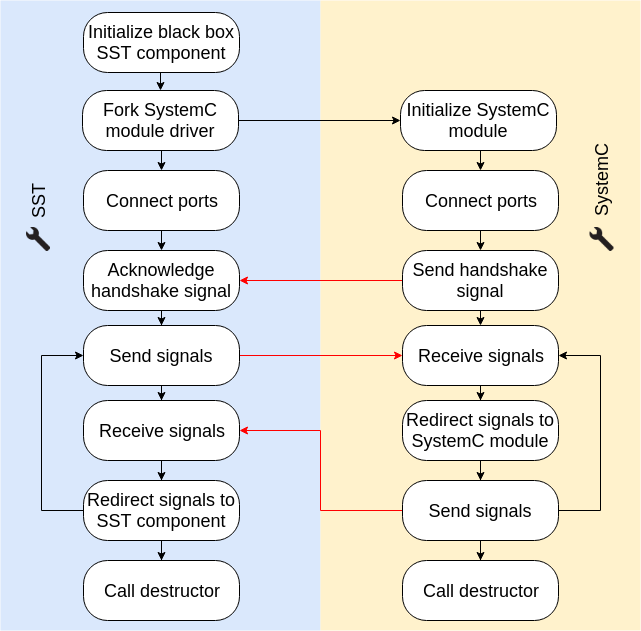
\includegraphics[width=5in]{diagrams/data_flow.png}
    \caption{Black Box Interface Data Flow Diagram; Arrows Highlighted in Red Indicate
    Communication Signals}
    \label{fig:data_flow}
  \end{figure}

    \subsection{Inter-Black Box Communication} \label{sec:ipc}
    The data is serialized into a string buffer with the substring positions and lengths generated
    by the Boilerplate Code Generator. The components inside the black box interface are spawned in
    the same node and therefore communicate via interprocess communication (IPC) transports. The
    following is a list of supported IPC transports:
    \begin{enumerate}
      \item Unix domain sockets
      \item ZeroMQ
    \end{enumerate}

    It is possible to integrate additional IPC protocols to the interface such as named pipes and
    shared memories.

    \subsection{SST-Black Box Communication}
    SST links are used to interface the SST component with the black box. The data is received as a
    \lstinline{SST::Interfaces::StringEvent} object which is casted to a standard string. SIT
    provides a custom event handler as part of its black box interface to allocate the substring
    positions and lengths for the ports.

    \subsection{HDL-Black Box Communication}
    The HDL module utilizes its program specific mechanism of communication to interface the black
    box driver. The method may be source file inclusion or importing modules.

%   \section{Proof of Concept: Traffic Intersection Simulation}
%   A simulation model has been developed to demonstrate the project. The model simulates a traffic
%   intersection controlled by two traffic lights. A flow of traffic is simulated through a road only
%   when its traffic light generates a green or yellow light with the other generating a red light.
%   The number of cars in a traffic flow is represented by random number generators.

%   \begin{figure}[!h]
%     \centering
%     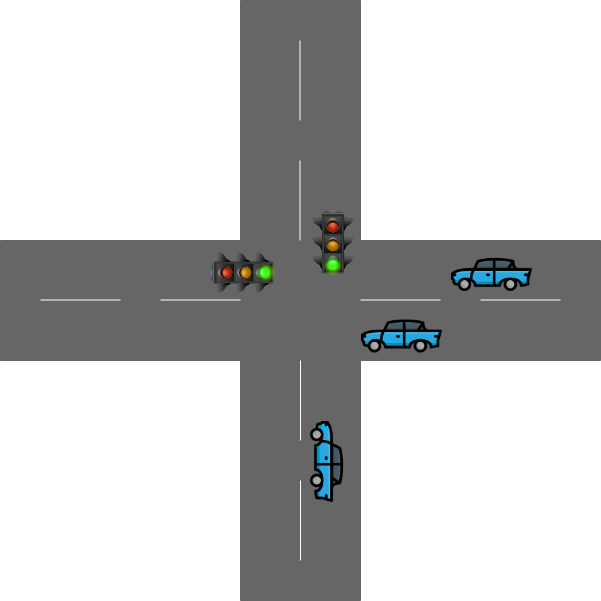
\includegraphics[width=3.5in]{diagrams/intersection.png}
%     \caption{Simple Two-Road Intersection}
%     \label{fig:intersection}
%   \end{figure}

%   The concept of this simulation is derived from the original project that established
%   interoperability between SST and PyRTL. \cite{pyrtl-sst}

%     \subsection{SystemC and PyRTL Drivers}
%     The simulation project includes a SystemC module and a PyRTL module with identical
%     functionalities. Their corresponding drivers interact with the SST component
%     \lstinline{traffic_light}. The module is a clock-driven FSM of three states representing the
%     three colors of a traffic light: green, yellow and red. The FSM proceeds to the next state when
%     indicated by its internal counter initialized in the beginning. The input variables to the
%     module include: the three durations for the three colors of the light, \lstinline{green_time},
%     \lstinline{yellow_time} and \lstinline{red_time}, the preset variable \lstinline{load} to
%     initialize the FSM, and \lstinline{start_green} to indicate if the first state should be
%     ``green'' or ``red''.

%     \begin{figure}[!h]
%       \centering
%       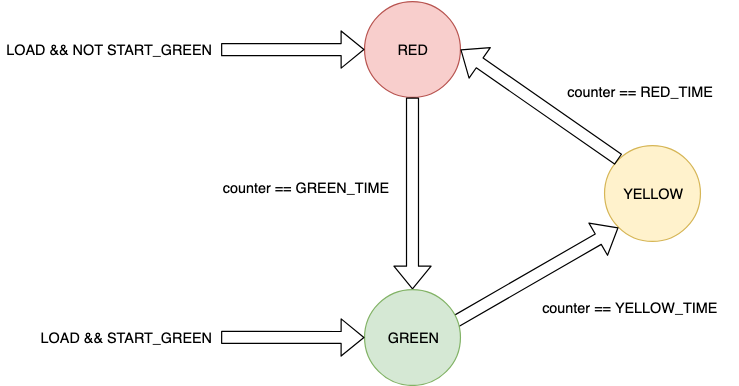
\includegraphics[width=4in]{diagrams/fsm.png}
%       \caption{Traffic Light Finite State Machine}
%       \label{fig:fsm}
%     \end{figure}

%     \subsection{SST Components}
%     The project also consists of three SST components: \lstinline{car_generator},
%     \lstinline{traffic_light_controller} and \lstinline{intersection}. All the components with the
%     exception of most of \lstinline{traffic_light_controller} were inherited from the original
%     project.

%       \begin{figure}[!h]
%         \centering
%         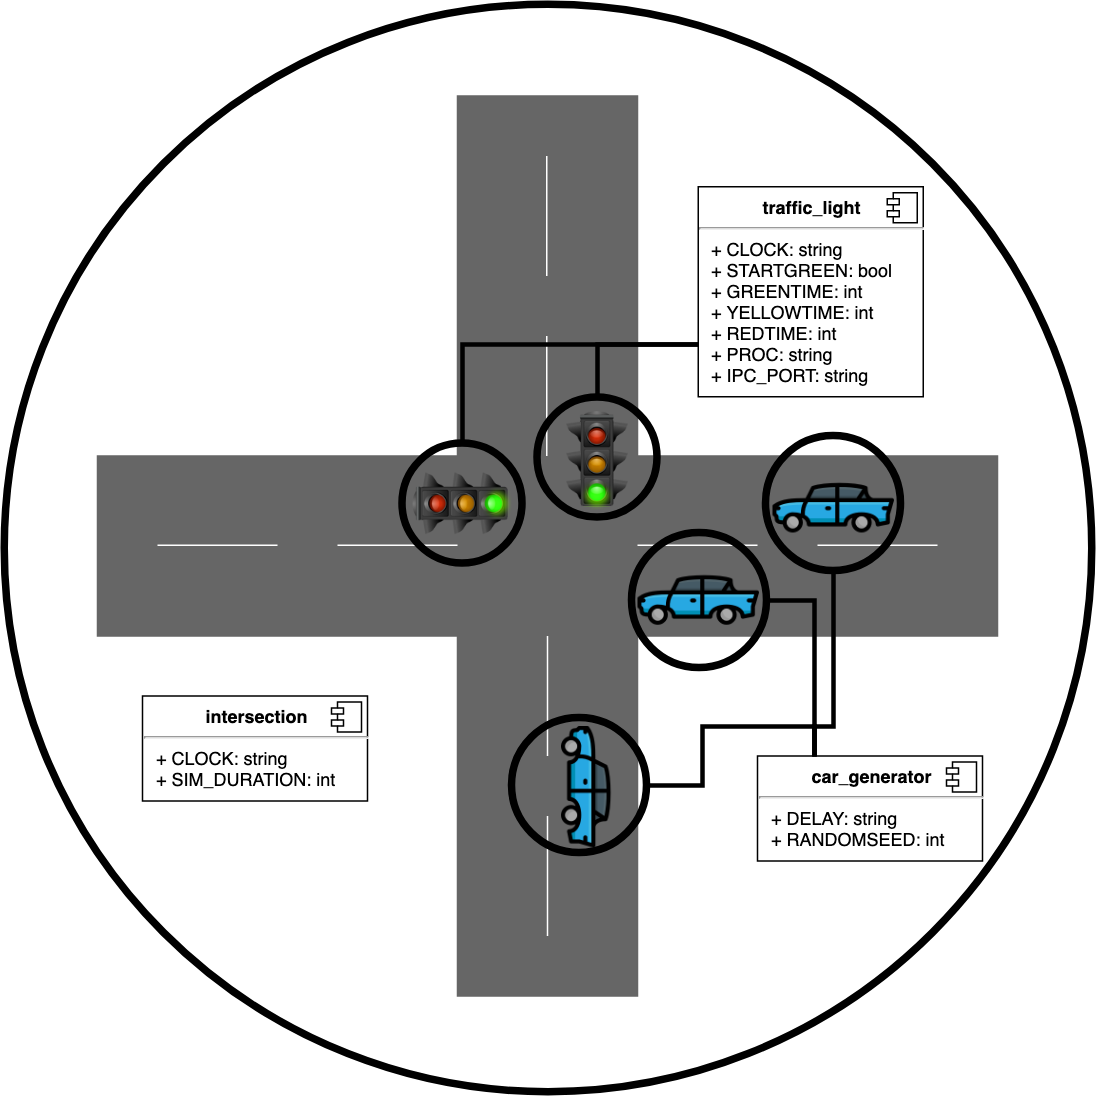
\includegraphics[width=4.5in]{diagrams/intersection_comp.png}
%         \caption{Simple Two-Road Intersection Represented by SST Components}
%         \label{fig:intersection_comp}
%       \end{figure}

%       \subsubsection{car\_generator}
%       The \lstinline{car_generator} component consists of a random number generator that yields $0$
%       or $1$. The output is redirected to \lstinline{intersection} via SST links.

%       \subsubsection{traffic\_light}
%       The \lstinline{traffic_light} component generates the light colors of the traffic lights using
%       a simple finite state machine (FSM). The component delegates the FSM portion of its algorithm
%       to the HDL module \lstinline{traffic_light_fsm} and inter-procedurally communicates with
%       it via Unix domain sockets. The component initializes the FSM with the SST parameters and
%       sends its output to \lstinline{intersection} via SST links every clock cycle.

%       \subsubsection{intersection}
%       \lstinline{intersection} is the main driver of the simulation. The component is able to handle
%       $n$ instances of \lstinline{traffic_light} subcomponents and therefore expects the same number
%       of \lstinline{car_generator} instances. For the purposes of this simulation, two instances of
%       the subcomponent pairs are set up. The driver keeps track of the number of cars generated and
%       the color of the light per clock cycle for each subcomponent pairs and stores them in local
%       variables. The variables are summarized in the end to generate statistics about the
%       simulation.

%       The component does not check for any collisions in the intersection, i.e. comparing if both
%       the \lstinline{traffic_light} subcomponents yield ``green'' during the same clock cycle. The
%       SST Python module is responsible for setting up the \lstinline{traffic_light} components with
%       the proper initial values.

%     \subsection{Example Simulation}
%     A sample output of the simulation has been generated and provided below. The SST components were
%     linked along with the parameters in the SST Python module.

% \begin{lstlisting}[caption={Sample Simulation Output}, captionpos=b]
% <@\textcolor{dkgreen}{traffic\_light-Traffic (SystemC) ->}@> GREENTIME=30, YELLOWTIME=3, REDTIME=63, STARTGREEN=0
% <@\textcolor{dkgreen}{traffic\_light-Traffic (PyRTL) ->}@> GREENTIME=60, YELLOWTIME=3, REDTIME=33, STARTGREEN=1
% <@\textcolor{mauve}{car\_generator-Car Generator 0 ->}@> Minimum Delay Between Cars=3s, Random Number Seed=151515
% <@\textcolor{mauve}{car\_generator-Car Generator 1 ->}@> Minimum Delay Between Cars=5s, Random Number Seed=239478
% <@\textcolor{blue}{intersection-Intersection ->}@> sim_duration=24 Hours
% <@\textcolor{blue}{intersection-Intersection ->}@> Component is being set up.
% <@\textcolor{dkgreen}{traffic\_light-Traffic (SystemC) ->}@> Component is being set up.
% <@\textcolor{dkgreen}{traffic\_light-Traffic (SystemC) ->}@> Forking process "/path/to/traffic_light_fsm.o"...
% <@\textcolor{dkgreen}{traffic\_light-Traffic (SystemC) ->}@> Process "/path/to/traffic_light_fsm.o" successfully synchronized
% <@\textcolor{dkgreen}{traffic\_light-Traffic (PyRTL) ->}@> Component is being set up.
% <@\textcolor{dkgreen}{traffic\_light-Traffic (PyRTL) ->}@> Forking process "/path/to/traffic_light_fsm.o"...
% <@\textcolor{dkgreen}{traffic\_light-Traffic (PyRTL) ->}@> Process "/path/to/traffic_light_fsm_driver.py" successfully synchronized
% <@\textcolor{blue}{intersection-Intersection ->}@> --------------------------------------
% <@\textcolor{blue}{intersection-Intersection ->}@> -------- SIMULATION INITIATED --------
% <@\textcolor{blue}{intersection-Intersection ->}@> --------------------------------------
% <@\textcolor{blue}{intersection-Intersection ->}@> Hour | Total Cars TL0 | Total Cars TL1
% <@\textcolor{blue}{intersection-Intersection ->}@> -----+----------------+---------------
% <@\textcolor{blue}{intersection-Intersection ->}@>    1 |              618 |            369
% <@\textcolor{blue}{intersection-Intersection ->}@>    2 |             1238 |            719
% <@\textcolor{blue}{intersection-Intersection ->}@>    3 |             1851 |           1074
% <@\textcolor{blue}{intersection-Intersection ->}@>    4 |             2432 |           1426
% <@\textcolor{blue}{intersection-Intersection ->}@>    5 |             3041 |           1774
% <@\textcolor{blue}{intersection-Intersection ->}@>    6 |             3688 |           2121
% <@\textcolor{blue}{intersection-Intersection ->}@>    7 |             4290 |           2467
% <@\textcolor{blue}{intersection-Intersection ->}@>    8 |             4892 |           2813
% <@\textcolor{blue}{intersection-Intersection ->}@>    9 |             5467 |           3175
% <@\textcolor{blue}{intersection-Intersection ->}@>   10 |             6054 |           3525
% <@\textcolor{blue}{intersection-Intersection ->}@>   11 |             6644 |           3885
% <@\textcolor{blue}{intersection-Intersection ->}@>   12 |             7228 |           4233
% <@\textcolor{blue}{intersection-Intersection ->}@>   13 |             7813 |           4607
% <@\textcolor{blue}{intersection-Intersection ->}@>   14 |             8435 |           4973
% <@\textcolor{blue}{intersection-Intersection ->}@>   15 |             9047 |           5337
% <@\textcolor{blue}{intersection-Intersection ->}@>   16 |             9656 |           5691
% <@\textcolor{blue}{intersection-Intersection ->}@>   17 |            10255 |           6059
% <@\textcolor{blue}{intersection-Intersection ->}@>   18 |            10843 |           6428
% <@\textcolor{blue}{intersection-Intersection ->}@>   19 |            11448 |           6791
% <@\textcolor{blue}{intersection-Intersection ->}@>   20 |            12025 |           7140
% <@\textcolor{blue}{intersection-Intersection ->}@>   21 |            12617 |           7499
% <@\textcolor{blue}{intersection-Intersection ->}@>   22 |            13225 |           7867
% <@\textcolor{blue}{intersection-Intersection ->}@>   23 |            13807 |           8223
% <@\textcolor{blue}{intersection-Intersection ->}@>   24 |            14400 |           8580
% <@\textcolor{blue}{intersection-Intersection ->}@> 
% <@\textcolor{blue}{intersection-Intersection ->}@> -------------------------------------------
% <@\textcolor{blue}{intersection-Intersection ->}@> ---------- SIMULATION STATISTICS ----------
% <@\textcolor{blue}{intersection-Intersection ->}@> -------------------------------------------
% <@\textcolor{blue}{intersection-Intersection ->}@> Traffic Light | Total Cars | Largest Backup
% <@\textcolor{blue}{intersection-Intersection ->}@> --------------+------------+---------------
% <@\textcolor{blue}{intersection-Intersection ->}@>              0 |       14400 |              18
% <@\textcolor{blue}{intersection-Intersection ->}@>              1 |        8581 |               7
% <@\textcolor{blue}{intersection-Intersection ->}@> Destroying Intersection...
% <@\textcolor{mauve}{car\_generator-Car Generator 1 ->}@> Destroying Car Generator 1...
% <@\textcolor{mauve}{car\_generator-Car Generator 0 ->}@> Destroying Car Generator 0...
% <@\textcolor{dkgreen}{traffic\_light-Traffic (SystemC) ->}@> Destroying Traffic (SystemC)...
% <@\textcolor{dkgreen}{traffic\_light-Traffic (PyRTL) ->}@> Destroying Traffic (PyRTL)...
% Simulation is complete, simulated time: 86.4 Ks
% \end{lstlisting}

  \section{Extensibility}

    \subsection{Communication}
    As mentioned in Section \ref{sec:ipc}, it is possible to integrate additional IPC protocols to
    the interface by implementing a derived class of \lstinline{sigutils::SignalIO} with customized
    sending and receiving methods. The base \lstinline{sigutils::SignalIO} class provides methods of
    serializing and deserializing the data structures utilized within the black box interface. The
    derived sending and receiving methods would have to simply implement their specific approaches
    of reading and flushing buffers.

    \subsection{Interface}
    This entire paper focuses on the interoperability established between SST and SystemC processes.
    However, the concept was derived off of the efforts already established by the SST-PyRTL project
    \cite{pyrtl-sst}. In fact, a hybrid version of the Traffic Intersection Simulation has been
    implemented where both SystemC and PyRTL take control over one traffic light using the same IPC
    method. The black box SST component had to be provided distinct instructions to spawn and
    communicate with a SystemC and a non-SystemC process. Meanwhile, the other side of the black box
    interface consisted of a SystemC driver and a PyRTL driver with their respective native
    configurations for establishing communication with the parent process.

    This extensibility was possible due to the generic structure of the black box interface. In
    theory, the interface is able to establish interoperability between SST and almost any other
    synthesizable HDL.


  \begin{thebibliography}{5}

    \bibitem{sst} SST Simulator - The Structural Simulation Toolkit. \texttt{sst-simulator.org}.

    \bibitem{pyrtl-sst} Mrosky, Robert P, et al.
    \textit{Creating Heterogeneous Simulations with SST and PyRTL}.

  \end{thebibliography}

\end{document}
